\chapter{Návrh riešenia}
\label{kap:navrh} % id kapitoly pre prikaz ref

\section{Návrh ontológie}

\begin{figure}[h]
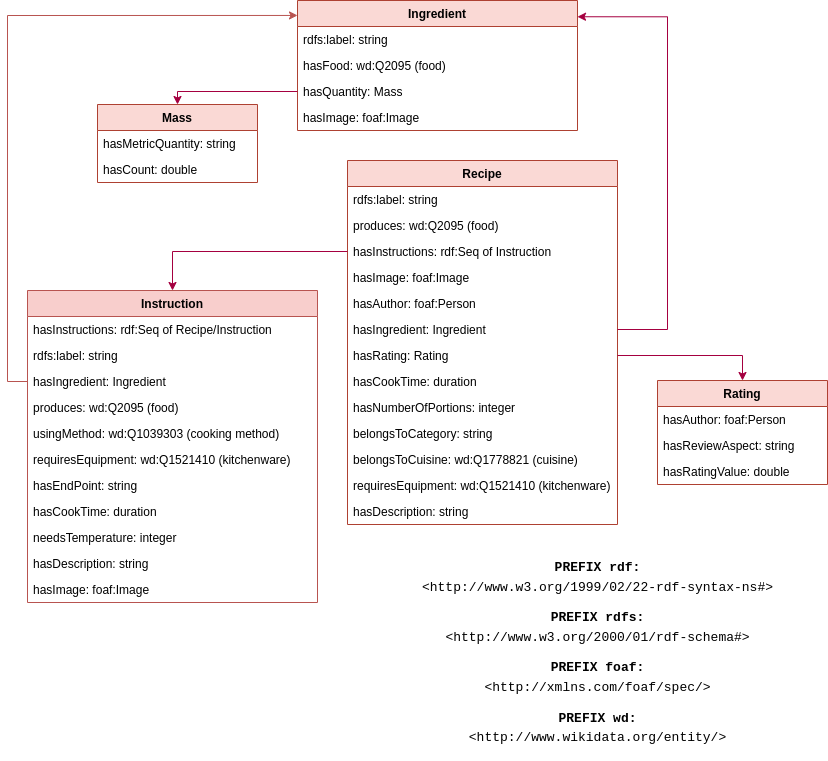
\includegraphics[width=\textwidth]{images/ontology}
\caption{Grafické vyjadrenie návrhu ontológie o receptoch}
\label{ontology}
\end{figure}

\subsection{Protégé}
Na vytvorenie ontológie sme využili Protégé, ktorý je možné stiahnuť na stránke \href{https://protege.stanford.edu/}{https://protege.stanford.edu/}. Protégé poskytuje grafické používateľské rozhranie, je to voľne dostupný editor ontológií a framework pre budovanie inteligentných systémov. Umožňuje modelovať triedy, predikáty, či vytvárať obmedzenia na jednotlivé predikáty. Následne je možné uložiť takto vytvorenú ontológiu v niektorej zo syntaxí pre jazyk OWL. Pri tvorbe našej ontológie sme využívali túto základnú funkcionalitu.

\subsection{Existujúca ontológia}
	Naša ontológia nadväzuje na ontológiu o receptoch v minuloročnej bakalárskej práci \cite{bakalarka}. Hlavnou úlohou bolo rozšíriť pôvodnú ontológiu o triedu, respektíve triedy, ktoré budú reprezentovať jednotlivé kroky (inštrukcie) v postupe receptu, keďže predtým bol postup iba pole reťazcov. V priebehu tvorby ontológie však došlo aj k ďalším menším zmenám v existujúcich triedach. Zároveň boli z pôvodnej ontológie odstránené triedy ingredientList a Food. Trieda ingredientList iba zapuzdrovala všetky ingrediencie patriace ku konkrétnemu receptu a trieda Food, ktorá vyjadrovala už existujúcu triedu a v našom prípade nebolo potrebné k nej pridávať žiaden ďalší predikát.
	
\subsection{Navrhnutá ontológia} \label{secOntologia}
Nižšie je popísaná ontológia podľa obr. \ref{ontology}. Pri popisovaní ontológie je v zátvorkách uvedený presný názov predikátu tak, ako sa nachádza v ontológií a v jej grafickom vyjadrení na obr. \ref{ontology}. V pravom dolnom rohu obr. \ref{ontology} sú uvedené využité prefixy v prípade, že trieda alebo predikát boli prevzaté z už existujúceho slovníka. 
	
\subsubsection{Popis tried existujúcich v predchádzajúcej ontológií}
	Hlavnou triedou je trieda Recipe, ktorá popisuje recept ako celok. Každý recept môže mať priradený obrázok (hasImage), názov vytváraného receptu zrozumiteľný pre používateľa (rdfs:label), autora (hasAuthor), čas potrebný na prípravu (hasCookTime), počet porcií, ktoré daný recept vytvára (hasNumberOfPortions), stručný popis, ktorý však ešte nepatrí k postupu (hasDescription) a môžnosť zaradiť recept do nejakej kategórie (belongsToCategory), pričom tento predikát môže byť použitý opakovane v prípade, že recept patrí do viacerých kategórií. Ďalšími predikátmi sú príslušnosť k nejakej národnej kuchyni (belongsToCuisine), požadované kuchynské potreby (requiresEquipment), hodnotenia daného receptu inými používateľmi (hasRating). V tom prípade je objektom inštancia triedy Rating, pričom každé hodnotenie má autora(hasAuthor) a môže obsahovať nejaký slovný komentár (hasReviewAspect) alebo číselne vyjadrenú spokojnosť s receptom (hasRatingValue). Každý recept vytvára nejaké jedlo, ktoré sa v niektorých prípadoch môže použiť ako ingrediencia v inom recepte, a preto bolo potrebné recept zaradiť aj do triedy Food (produces). Toto zaradenie nám ďalej aj umožňuje vyhľadávať recepty, ktoré vytvárajú rovnaké jedlo.
	
	Predikát umožňujúci priradzovať k danému receptu ingrediencie (hasIngredient) spája triedu Recipe s triedou Ingredient. Každá ingrediencia môže mať názov zrozumiteľný pre používateľa (rdfs:label), obrázok (hasImage), jednotku merania (hasMetricQuantity), množstvo (hasCount), pričom posledné 2 spomenuté predikáty patria triede Mass. Každá ingrediencia je nejaké už existujúce jedlo (hasFood).
	
\subsubsection{Popis triedy Instruction}
	Každý recept musí mať nejaký postup (hasInstructions). Objektom tohto predikátu je kontainer rdf:Seq, ktorý sa používa v prípadoch, kedy potrebujeme poznať poradie pridávaných položiek. V tomto prípade je možné do kontainera pridávať inštancie triedy Instruction.
	
	Pri definovaní krokov v postupe receptu sme uvažovali nad viacerými možnosťami ako ich vytvárať. Plánovali sme oddeľovať triedu Description, Stage a Step, vďaka ktorým by sa dal recept pekne rozčleniť. Avšak nie každý recept má takúto štruktúru a pri iných typoch receptov by boli častokrát zbytočné triedy Stage, či Description. V prípade samotného kroku sme uvažovali nad tým, že bude obsahovať triedu Activity, ktorá presne popíše, ktorú surovinu, akým spôsobom, a za akých podmienok bude spracovávať. Toto by síce dokonale rozobralo každý krok receptu, avšak praktické využitie takto podrobnej ontológie by bolo príliš náročné. 
	
	Rozhodli sme sa preto pre možnosť vytvoriť jedinú triedu Instruction. Inštrukcia môže zaobaľovať celú postupnosť krokov k receptu, môže vyjadrovať nejakú časť krokov, ktoré tvoria samostatnú časť jedla, napr. v prípade koláča to je inštrukcia na vytvorenie plnky, cesta, či polevy, alebo môže inštrukcia vyjadrovať jediný krok. Využitie triedy bude teda závisieť od toho, ako bude vyzerať postup k receptu. Práve kvôli rôznorodosti postupov sme museli vytvoriť dostatočne všeobecnú triedu, aby mohla umožniť rovnako ľahko vytvoriť recept s jedným krokom, ako aj recept s pomerne zložitým postupom, v ktorom sú isté časti receptu oddelené do samostatných celkov. Používateľovi je umožnené priradiť techniku prípravy, ktorú je potrebné využiť pri danom kroku (usingMethod), napr. vyprážanie, pečenie, možnosť priradiť obrázok (hasImage), názov (rdfs:label), teplotu, pri ktorej má byť daná inštrukcia vykonávaná (needsTemperature), požadované kuchynské potreby (requiresEquipment), či potraviny spracovávané v danej časti receptu (hasIngredient).  Trieda Instruction ďalej umožňuje vyjadriť čas potrebný na vykonanie nejakého kroku (hasCookTime). V niektorých prípadoch je trvanie kroku vyjadrené slovne, napr. pečieme, kým nezhnedne, vtedy použijeme predikát, ktorý vyjadruje práve prechod ingrediencie do nejakého finálneho stavu (hasEndPoint). Ak ide o skupinu krokov, ktoré vytvárajú celý postup k receptu alebo časť receptu, napr. prípravu cesta pri pečení koláča, využijeme predikát hasInstructions. Ten ako objekt obsahuje sekvenciu, pomocou rdf:Seq, ďalších inštrukcií alebo receptov v prípade, že by sme sa v nejakej časti receptu chceli odkázať na už existujúci recept. Ak chceme popisovať už koncový krok, ktorý sa skladá iba zo slovného popisu a ďalej sa nečlení, využijeme predikát hasDescription. V prípade, že nejaká inštukcia vytvára jedlo, môžeme využiť predikát produces.
 
\section{Funkcionalita systému} \label{secFunkcionalitaSystemu}
V tejto podkapitole popisujeme funkcionalitu systému. Ide o prehľad toho, čo používateľ môže využívať v prípade, že túto webovú aplikáciu navštívi.

\begin{enumerate}
\item \textbf{Registrácia používateľa} - Používateľ má možnosť sa zaregistrovať vyplnením formulára, kde je nutné uviesť používateľské meno a heslo. 

\item \textbf{Prihlásenie používateľa} - Prihlásenie do aplikácie prebieha prostredníctvom rovnakého formulára ako registrácia, teda stačí vylpniť používateľské meno a heslo, pričom po prihlásení získa používateľ prístup k dovtedy neprístupným stránkam, ktorými sú vytváranie nového receptu a zoznam jeho vlastných receptov.

\item \textbf{Zobrazenie všetkých receptov aj pre neprihlásených používateľov} - Používateľ si môže zobraziť všetky recepty naraz, pričom ku každému receptu bude vidieť jeho názov a popis. 

\item \textbf{Vyhľadávanie receptov aj pre neprihlásených používateľov podľa:} 
\begin{itemize}
\item \textbf{názvu} - Používateľ má možnosť vyhľadať recept zadaním jeho názvu. Vyhľadávané sú všetky recepty, ktorých časť názvu sa zhoduje s tým, čo používateľ zadal do vyhľadávacieho okna.
\item \textbf{dĺžky prípravy}- Používateľ má možnosť zvoliť si interval dĺžky prípravy jedla, teda iba spodnú hranicu, iba hornú hranicu, alebo obidve naraz. 
\item \textbf{ingrediencií}  
\item \textbf{autora}  
\item \textbf{národnej kuchyne} 
\item \textbf{spôsobu prípravy jedla} 
\item \textbf{kuchynských potrieb} 
\item \textbf{kategórie} 
\end{itemize}

V prípade vyhľadávania podľa ingrediencií, autora, národnej kuchyne, spôsobu prípravy jedla, kuchynských potrieb a kategórie má používateľ možnosť uviesť položky z jednotlivých skupín, ktoré má recept obsahovať aj ktoré obsahovať nemá. 

V prípade vyhľadávania podľa ingrediencií, autora, národnej kuchyne, spôsobu prípravy jedla, kuchynských potrieb a kategórie, ak používateľ uvedie jednu alebo viacero položiek, ktoré recept nemá obsahovať, z výsledných receptov budú odstránené všetky, ktoré aspoň jednu z týchto  položiek obsahujú. 

V prípade vyhľadávania podľa ingrediencií, autora, národnej kuchyne, spôsobu prípravy jedla, kuchynských potrieb a kategórie, ak používateľ uvedie jednu alebo viacero položiek, ktoré recept musí obsahovať má možnosť zvoliť si jeden z dvoch spôsobov vyhľadávania pri každej z týchto skupín. Pri prvom spôsobe sa vo výsledných receptoch objavia len tie recepty, ktoré obsahujú všetky položky, ktoré používateľ chce zahrnúť zároveň alebo druhý spôsob, pri ktorom obsahujú výsledné recepty aspoň jednu z položiek (napr. ak používateľ chce v recepte ryžu a kuracie mäso, pri prvom spôsobe budú vyhľadávané tie recepty, ktoré obsahujú obe ingrediencie a pri druhom recepty, ktoré obsahujú aspoň jednu z nich).

Položky zadané používateľom budú porovnávané rovnako ako názov v bode 1, teda vybrané, respektíve odstránené budú tie recepty, v ktorých sa časť názvu položky vybranej skupiny v recepte zhoduje s tým, čo používateľ zadal. 

\item \textbf{Zobrazenie receptu} - Každý používateľ, prihlásený aj neprihlásený, si môže zobraziť podrobnosti o recepte, ktoré autor receptu pri vytváraní zadal. Keďže pri receptoch ide o rôznorodé dáta, ktoré môžu mať uvedené rôzne vlastnosti, zobrazované budú len tie údaje, ktoré používateľ vo formulári pri vytváraní receptu  vyplnil. Nevyplnené položky sa pri zobrazení odignorujú. Pri každom recepte sa budú zobrazovať rovnaké, respektíve podobné recepty, na základe jedla, ktoré autor uviedol pri vytváraní receptu pri vlastnosti produces. 

\item \textbf{Pridanie vlastného receptu} - Každý prihlásený používateľ má možnosť vytvoriť vlastný recept, ktorého ako autor bude figurovať, teda každý recept má práve jedného autora. Povinnými poliami pre vytvorenie receptu sú názov, popis, jedlo, ktoré recept vyprodukuje, pričom to musí byť jedlo zahrnuté v databáze, aspoň jedna ingrediencia, a aspoň jeden krok v postupe. Ďalej je možné uviesť počet porcií, čas potrebný na prípravu, kategórie a národné kuchyne do ktorých recept patrí, kuchynské potreby nutné na prípravu a spôsoby prípravy. Pri vypĺňaní postupu receptu je možné uvádzať kroky aj podkroky. Ak má krok podkroky, v tom prípade je nutné uviesť názov celého kroku. Používateľ má možnosť uviesť pri jednotlivých krokoch a podkrokoch aj ingrediencie, spôsoby prípravy, kuchynské potreby, čas potrebný na prípravu alebo popis stavu, v ktorom daný krok,respektíve podkrok končí, teplotu a takisto jedlo, v prípade, že krok vytvára niečo, čo môžme označiť za hotové jedlo. 

\item \textbf{Úprava vlastného receptu} - Jednotlivé časti receptu môže používateľ upraviť po kliknutí na tlačidlo Edit, ktoré sa mu však zobrazí iba v prípade, že sa nachádza v časti stránky so zoznamom jeho vlastných receptov. V tom prípade sa používateľovi zobrazí recept v takej forme ako keď je vytváraný, avšak všetky polia budú predvyplnené. Ak po úprave ostanú vyplnené všetky povinné polia, úprava sa bude považovať za úspešnú.

\item \textbf{Možnosť zobraziť si všetky národné kuchyne, metódy prípravy, kuchynské potreby a jedlá (ingrediencie) zahrnuté v databáze} - Aj neprihlásený používateľ si môže zobraziť jeden zo zoznamov, ktorý obsahuje všetky položky z vybranej kategórie. Tieto položky (entity) sú prebrané z wikidata, pričom ich používateľ využíva pri vytváraní receptu v poliach, v ktorých pridáva názov ingrediencie, spôsobu prípravy, kuchynskej potreby a národnej kuchyne.

\item \textbf{Možnosť zistiť bližšie informácie o jedle (ingrediencií), národnej kuchyni, spôsobe prípravy a vybranej kuchynskej potrebe} - 
Ak sa používateľ dostane do zoznamu nejakej z uvedených kategórií (funkcionalita z bodu 8), o každej z položiek má možnosť dozvedieť sa viac. Po kliknutí na položku sa mu zobrazia informácie, ktoré sú o nej dostupné na stránke wikidata vo forme tabuľky s dvoma stĺpcami property a value. Každá vlastnosť (property) a jej hodnota (value) je odkazom, takže sa používateľ dostane aj k ďalším podrobnejším informáciám, avšak bude už presmerovaný priamo na stránku wikidata, keďže to budú informácie, ktoré nie sú priamo viazané na recepty.  

\item \textbf{Odkazy pri prihlasovaní používateľa, detaile a vytváraní receptu} - Možnosť dozvedieť sa viac o nejakej entite nie je možné iba vyššie uvedeným spôsobom (funkcionalita z bodu 9). Pri vytváraní receptu aj pri prihlasovaní používateľa sú vo formulári pri všetkých poliach uvedené názvy, ktoré používateľovi hovoria, čo má do poľa zadať. Tieto názvy sú však aj odkazmi na ontológie, v ktorých je daná vlastnosť zadefinovaná, a teda kliknutím na nich sa používateľ dostane k ich podrobnejšiemu popisu. Pri detaile receptu, sa tu okrem odkazov na ontológie nachádzajú aj odkazy na triedy z wikidata, v prípade, že niektorá časť receptu tieto triedy obsahuje.   
\end{enumerate}

\section{Návrh databázy aplikácie}
Sú vytvorené dve databázy. Jedna databáza obsahuje informácie o používateľoch aplikácie, teda ich prihlasovacie údaje. Druhá databáza ukladá všetky recepty s informáciami, ktoré k nim boli uvedené. Informácie sú do databázy vkladané na základe vytvorenej ontológie (\ref{secOntologia}). Ďalej táto databáza obsahuje aj všetky entity importované z wikidata, teda ingrediencie, kuchynské potreby, spôsoby prípravy jedla a národné kuchyne. Ku každej z týchto 4 skupín je v databáze uložená vlastnosť rdfs:label, kvôli tomu, aby používateľovi mohla byť táto entita zobrazená s názvom, ktorému porozumie a zároveň s vlastnosťou rdfs:comment, ktorý hovorí o tom, do ktorej z týchto 4 skupín patrí. 

\section{Návrh backendu aplikácie}
Backend aplikácie zodpovedá za dopyty vytvárané nad databázou, umožňuje vytvárať triedy, ktoré sa budú zhodovať s triedami vo vytvorenej ontológií (\ref{secOntologia}) a poskytuje REST API rozhranie. Na obr. \ref{backend} vidíme vizualizáciu tried a balíčkov, ktoré budú zodpovedať za túto funkcionalitu.
\begin{figure}[h]
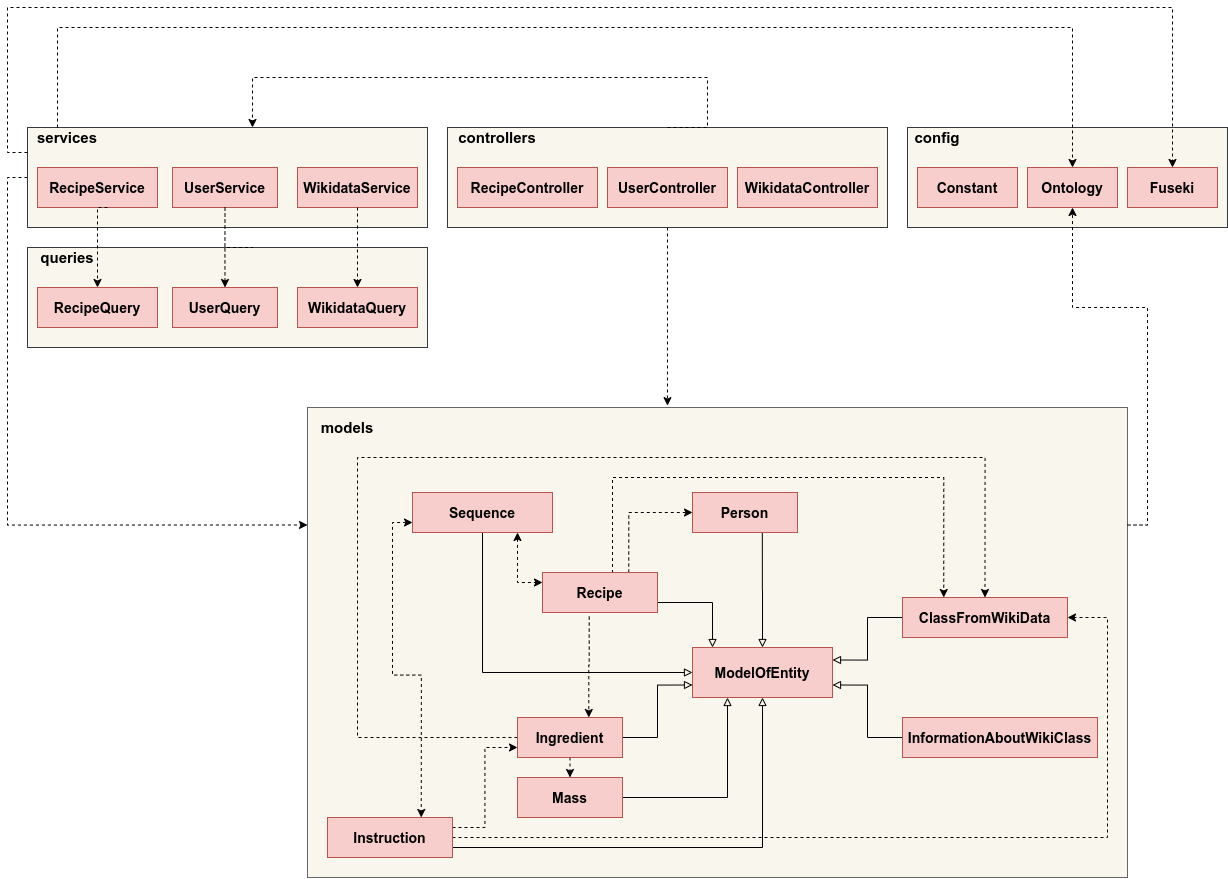
\includegraphics[width=\textwidth]{images/backend}
\caption{Vizualizácia štruktúry balíčkov a tried na backende}
\label{backend}
\end{figure}
Práca s databázou sa nachádza v balíčku services, pričom sú v ňom oddelené tri súbory na základe toho, aká entita má byť výsledkom ich dopytu. Tento balíček využíva balíček queries, ktorý zodpovedá za vytváranie potrebných dopytov a triedu Ontology a Fuseki. Fuseki zodpovedá za pripojenie sa na databázu, pričom toto pripojenie je opakovane používané a Ontology obsahuje ontológiu na základe ktorej s dátami pracujeme. REST API je vytvárané v balíčku controllers, čo teda znamená, že bude obsahovať triedy s metódami, ktoré budú obsluhovať URL adresy pre requesty, ktoré budú prichádzať. V balíčku models sa nachádzajú triedy, ktoré reprezentujú triedy z ontológie, pričom sú využívané v services a controllers ako návratové typy. 

\section{Návrh frontendu aplikácie}
Frontend vytvára používateľské rozhranie a teda umožňuje komunikovať používateľovi s aplikáciou. Grafické rozhranie aplikácie bude pozostávať z viacerých komponentov, ktoré sú v balíčku components. Sú to komponenty, ktoré sa používateľovi môžu zobraziť v prehliadači pričom ich úlohou je len čítať aktuálny stav aplikácie, na základe toho zobrazovať jednotlivé komponenty, a prípadne na základe určitej akcie od používateľa vytvoriť reakciu, teda spustiť funkciu, ktorá dokáže stav aplikácie zmeniť. Pre jednoduchšie priblíženie toho, aké komponenty v aplikácií vystupujú a ako sú medzi sebou prepojené si môžeme pozrieť obr. \ref{reactComponents}. 
\begin{figure}[h]
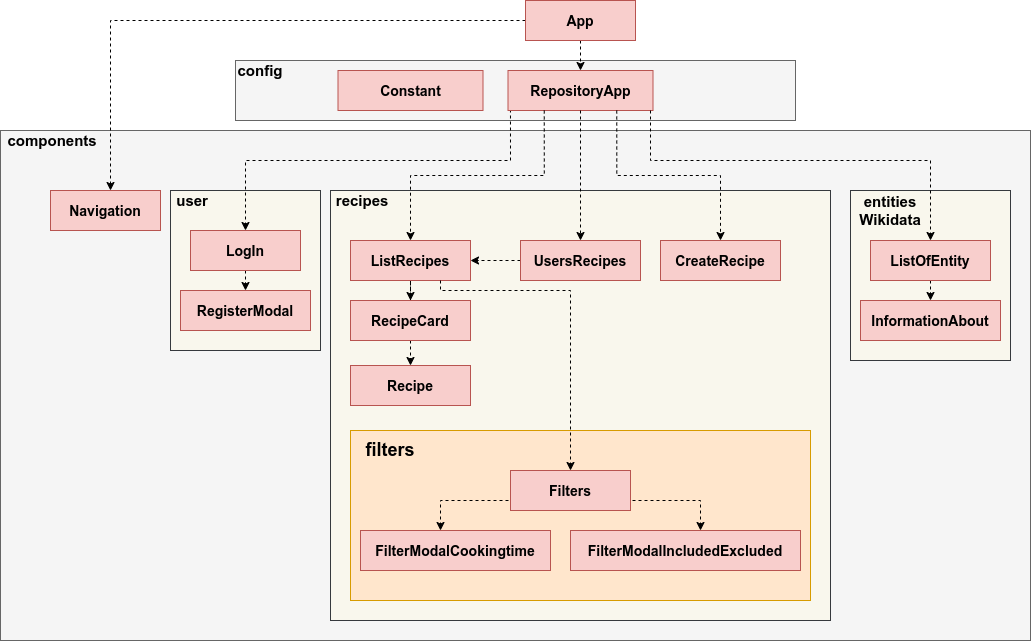
\includegraphics[width=\textwidth]{images/reactComponents}
\caption{Vizualizácia štruktúry balíčkov, komponentov a ich vzťahov na frontende}
\label{reactComponents}
\end{figure}
Jednotlivé komponenty sú roztriedené do balíčkov na základe funkcionality, ktorú plnia. Balíček user dáva možnosť registrácie alebo prihlásenia sa používateľovi, pričom poskytuje 1. a 2. bod z funkcionality systému (\ref{secFunkcionalitaSystemu}). Zobrazovanie zoznamov receptov, ich detailov, či ich vytváranie umožňuje balíček recipes, pričom je tu zahrnutá funkcionalita (\ref{secFunkcionalitaSystemu}) od 3.bodu až po bod 7. Filtrovanie receptov z bodu 4 je umožnené vďaka balíčku filters. Balíček entitiesWikidata zodpovedá za funkcionalitu systému(\ref{secFunkcionalitaSystemu}) z bodov 9 a 10, teda vďaka týmto komponentom má používateľ možnosť zobraziť si všetky triedy prevzaté z wikidata, prípadne detailné informácie o nich. Presmerovávanie medzi stránkami je vytvorené v RepositoryApp, pričom navigácia umožňuje používateľovi sa medzi týmito stránkami jednoducho prepínať. V súbore Constant sú uložené konštanty, ku ktorým má prístup celá aplikácia a môže ich v prípade potreby využívať. 

